

\section{Vektoren für die Klonierung von DNA}
Für das Prinzip der Klonierung siehe \ref{sec:klonierung}. \index{Klonierung}
\subsection{\glspl{plasmid}}
\subsubsection{E. coli-Plasmidvektoren: pBR322} \index{Plasmidvektoren}
\begin{itemize}
\item eines der ersten künstlich hergestellten \glspl{plasmid}
    \item Derivat eines R-(Resistenz-) \gls{plasmid}s
    \item Ampicillin-Resistenz aus Tn3
    \item \gls{tetracyclin}-Resistenz aus pSC101
    \item heutige pUC-\glspl{plasmid} sind Derivate von pBR322 \index{pBR322} \index{Plasmid!pUC}
\end{itemize}
\subsubsection{pUC-\glspl{plasmid}}
\begin{itemize}
    \item \gls{plasmid}serie
    \item multiple cloning site (MCS, \gls{Polylinker}) im lacZ-Gen \index{lacZ} \index{Polylinker} \index{multiple cloning site }
    \item high copy number-Plasmid
    \item Blau-Weiß-Screening \index{Blau-Weiß-Screening}
    \item relativ geringe Größe
    \item chromosomales LacZ$\Omega$ wird durch LacZ$\alpha$ komplementiert zur
aktiven $\beta$-Galactosidase \index{$\beta$-Galactosidase} \index{LacZ}
\end{itemize}
\begin{mybox}[title=Was ist Blau-Weiß-Screening?]
Methode, um Bakterienkolonien zu identifizieren, die ein rekombinantes \gls{plasmid} enthalten. \\ Bei der Klonierung wird das DNA-Fragment von Interesse in die multiple Klonierungsstelle (MCS) des Plasmids inseriert, die sich innerhalb des lacZ$\alpha$-Gens befindet. Wenn das Insert erfolgreich in das lacZ$\alpha$-Gen eingefügt wird, wird die Produktion von funktioneller $\beta$-Galactosidase unterbrochen, da das lacZ$\alpha$-Fragment nicht mehr intakt ist. \\
Kolonien, die das rekombinante \gls{plasmid} mit einem Insert tragen, können keine funktionelle $\beta$-Galactosidase produzieren und bleiben daher weiß. Kolonien, die das \gls{plasmid} ohne Insert tragen, produzieren funktionelle $\beta$-Galactosidase und erscheinen blau, da sie \gls{X-Gal} in das blaue Produkt umwandeln. \index{X-Gal} \index{lacZ} \index{$\beta$-Galactosidase}
\end{mybox}
\begin{mechanism}[title=Was macht X-Gal?]
Enzym; Kann von $\beta$-Galactosidase gespalten werden und daraus entsteht ein blauer Farbstoff. So kann man $\beta$-Galactosidase nachweisen. (Blau-Weiß-Screening)
\end{mechanism}
\subsubsection{Alpha-Komplementation der $\beta$-Galaktosidase}
\begin{itemize}
    \item \textbf{$\beta$-Galaktosidase} ist ein Homotetramer, das aus vier identischen Untereinheiten besteht. \index{$\beta$-Galaktosidase}
    \item \textbf{Alpha-Komplementation} erfordert spezielle E. coli-Stämme mit einer Mutation im lacZ-Gen, wie z.B. JM109, DH5$\alpha$ oder XL1-Blue. \index{lacZ} \index{Alpha-Komplementation}
    \item Der Mutationsstamm \textit{lacZ$\Delta$M15} hat eine Deletion der Aminosäuren 11 bis 41, was zur Bildung des \textit{$\omega$}-Peptids führt, das keine Homotetramerbildung ermöglicht.
    \item Das \textit{$\alpha$}-Peptid, bestehend aus den Aminosäuren 1 bis 59, ergänzt das \textit{$\omega$}-Peptid und bildet eine funktionsfähige $\beta$-Galaktosidase.
    \item Das \textit{$\alpha$}-Peptid wird auf einem \gls{plasmid} kodiert, das als \textit{lacZ$\alpha$} bezeichnet wird.
\end{itemize}


\subsection{Bakteriophagen}
\subsubsection{Auf Basis von E. coli-Bakteriophage $\lambda$}
Lambda kann eine Wirtszelle auf zwei Arten infizieren:  \index{Bakteriophage}
\begin{itemize}
    \item \textbf{Lytisch}: $\lambda$-DNA lässt die Wirtszelle direkt neue Phagen erstellen und die Wirtszelle stirbt
    \item \textbf{Lysogenisch}: Es wird erst Phagen-DNA in das Genom der Wirtszelle integriert und nach einigen Zellteilungen geht es in den lytischen Zyklus über 
\end{itemize}
Es gibt Insertionsvektoren und Austauschvektoren. Die zu transportierende DNA wird in beide Vektoren zwischen sog. Restriktionsschnittstellen (restriction sites) eingefügt. \\ \newline
Insertionsvektoren haben cos-Stellen an den Enden (Überhänge). Die sind relevant dafür, dass sich die DNA nach der Injektion zirkularisiert, denn nach Injektion in den Wirt hybridisieren die cos-Enden miteinander. Der Phagen-Verpackungsapparat erkennt cos-Stellen außerdem als Schnittsignal. \\ \index{Vektor!Insertions} \index{Vektor!Austauschs}
\noindent Vorgang:
\begin{itemize}
    \item Insertion eines DNA-Fragments in den \gls{vektor} \index{Vektor}
    \item Einbringen der Vektoren in E. coli
    \item Transformation (Transfektion)
    \item in vitro-Verpackung
    \item infizierte Zellen lysieren, sterben, neue Zellen werden infiziert
\end{itemize}

\index{Large-Insert-Klon}
\begin{mechanism}[title=Eigenschaften für Vektoren mit large-insert Klonen. Nennen sie zwei Beispiele.]
\begin{itemize}
    \item Hohe Kapazität (bp)
    \item Origin of replication
    \item Stabilität
\end{itemize}
BAC / YAC
\end{mechanism}
\begin{mechanism}[title=\gls{plasmid} Isolierung- Wie heißt dieser Vorgang?]
Klonierung
\end{mechanism}


\subsection{Cosmide, Fosmide, BACs und YACs}
\index{Cosmid} \index{Fosmid} \index{BAC} \index{YAC}
\begin{table}[H]
    \centering
    \begin{tabular}{p{2.5cm}p{3cm}p{3cm}p{3.25cm}p{3.25cm}}
        & \textbf{Cosmide} & \textbf{Fosmide} & \glspl{bac} & \glspl{yac} \\ \\ 
        \textbf{Basis} & $\lambda$-Phagen und \glspl{plasmid} & \textit{F-Plasmid} & \textit{F-Plasmid} & Chromosom \\ \\
        \textbf{Stabilität} & relativ instabil & \textit{Stabil} & \textit{Stabil} & 
        \textit{Stabil} \\ \\
        \textbf{Kopienzahl} & hoch & \textit{niedrig} (1) & \textit{niedrig} & \textit{niedrig} \\ \\
        \textbf{Partitio-nierungs-Funktionen} &  keine &  \textit{ja} & \textit{ja} & \textit{ja} \\ \\
        \textbf{Regulation der Kopienzahl} & keine & \textit{Partitionierungs-Gene }& \textit{Partitionierungs-Gene} & Centromer u. Telomere \\ \\
        \textbf{Vektor-Verpackung} & In Bakteriophagenpartikel & \textit{keine} & \textit{keine} & \textit{keine}  \\ \\
        \textbf{Fragmentlänge} & bis 44 kb & ca. 40 kb & bis ca. 300 kb & > 1400 kb \\ \\
        \textbf{Replizierung} & hybride Replikationsstrategie & \textit{wie \glspl{plasmid}} & \textit{wie \glspl{plasmid}} & wie Chromosomen \\  \\
        \textbf{Infektions-eigenschaften} & Ja, aber keine neuen Phagen & \textit{keine} & \textit{keine} & \textit{keine} \\ \\
        \textbf{Replikations-ursprung}&  $\lambda$-cos-Stellen \index{$\lambda$-cos-Stelle} (MCS) &  oriV \index{oriV} (MCS) & oriS \index{oriS} (MCS) & ori (MCS)\\ \\
    \textbf{Antibiotika-resistenzen} & \textit{Ja} & \textit{Ja} & \textit{Ja} & selten/keine \\ \\
    \textbf{lacZ$\alpha$} & kann in $\beta$-Galaktosidase-Fusionen verwendet werden & nein & Blau/Weiß-Screening (mcs) & nein \\ \\
    \textbf{Mechanimus} & \textit{Restriktionsenzyme} & \textit{Restriktionsenzyme} & \textit{Restriktionsenzyme} & homologe Rekombination 
    \end{tabular}
    \caption{Vergleich der Vektor-Eigenschaften von Cosmiden, Fosmiden, BACs und YACs.}
    \label{tab:cosfosacs}
\end{table}
BACs und YACs unterscheiden sich in ihrem Ursprung und das wirkt sich auf ihre Eigenschaften aus. Beide sind Large-Insert-Vektoren mit Regulation der Kopienzahl, stabiler Vererbung und einem \gls{Polylinker} (\gls{mcs}). \\
YACs sind Chromosomen nachempfunden und haben deren Regulationen zur stabilen Vererbung und Partitionierung: Centromere und Telomere (Centromere, weil da die Chromosomen getrennt werden) und BACs hingegen haben Partitionierungs-Gene. \\
YACs haben im Gegensatz zu BACs meistens keine Antibiotikaresistenzen und kein LacZ-Gen. 

\begin{mechanism}[title=Skizzieren sie einen BAC-Vektor]
\begin{figure}[H]
    \centering
    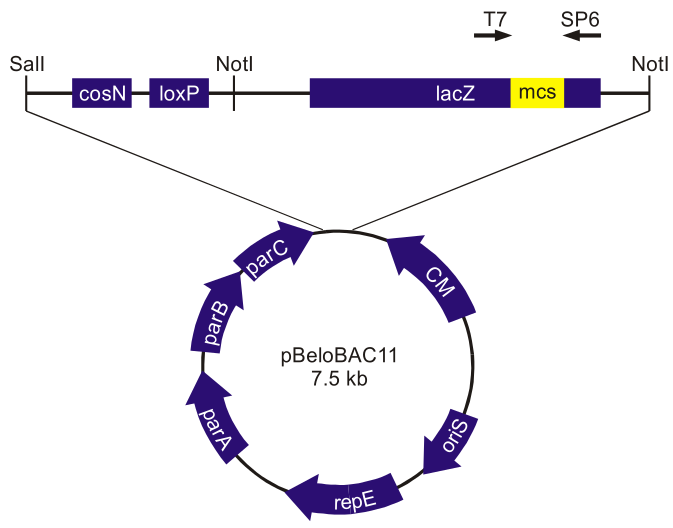
\includegraphics[width=10cm]{images/bacvector.png}
    \caption{\textbf{BAC-Vektor}: \textit{parA, parB, parC}: Aufteilung (partitioning) auf Tochterzellen während Zellteilung, stabile Weitergabe;  \textit{\gls{repe}}; \textit{CM}: Antibiotikaresistenz (Chloramphenicol)}
    \label{fig:bacvector}
\end{figure}
\end{mechanism}
\begin{mechanism}[title=Bennen Sie die wesentlichen Eigenschaften eines BAC-Vektors]
\begin{itemize}
    \item große Kapazität
    \item hat Replikationsursprung
    \item hat Selektionsmarker
    \item Stabile Vererbung
    \item MCS
\end{itemize}
\end{mechanism}
\begin{mybox}[title=Was hat keine MCS?]
\begin{itemize}
    \item Viele natürlich vorkommende Plasmide in Bakterien
    \item Die natürlichen Chromosomen von Organismen, sowohl prokaryotisch als auch eukaryotisch
\end{itemize}
\end{mybox}
\begin{mechanism}[title=Wofür setzt man einen BAC-Vektor ein?]
\begin{itemize}
    \item Klonierung großer DNA-Fragmente
    \begin{itemize}
        \item Genomkartierung
        \item Sequenzierung
        \item Studien zur genetischen Variation
    \end{itemize}
\end{itemize}
\end{mechanism}


\section{Konstruktion von genomischen Klon-Bibliotheken} \index{Klon-Bibliothek}
Berechnung der benötigten Klonanzahl (vermutlich nicht Klausurrelevant): \begin{equation*}
    \#\text{Klone} = 
    \frac{
    ln(1-\text{Wahrscheinlichkeit, dass Genomsegment in Bibliothek)}
    }
    {ln(1- 
    \frac{
    avg(\text{Größe des DNA Fragments})
    }{
    \text{Genomgröße}
    } )}
\end{equation*}
Genereller Ablauf: 
\begin{enumerate}
    \item Isolierung der genomischen DNA
    \item Fragmentierung der DNA
    \item Ligation der DNA-Fragmente in den Vektor
    \item Transformation in Wirtszellen
    \item Selektion von transformierten Zellen
    \item Screening und Speicherung
\end{enumerate}
\section{Strategien zur Sequenzierung von Genomen} \index{Sequenzierung}
Takeaway: Unterteilung des Genoms in Fragmente notwendig, die für Sequenzierung geeignet sind! \\ \newline 
Individuelle Sequenzen/Fragmente müssen anschließend wieder in ihre „native“ Anordnung gebracht werden und daher ist eine Überlappung untereinander notwendig, um die Stücke reassemblieren zu können. \\ \newline
$\Rightarrow$ heute häufig Kombination aus Whole genome shotgun-Sequenzierung und Ordered shotgun-Sequenzierung!

\begin{table}[H]
 \centering
\begin{tabular}{p{3cm}p{6cm}p{6cm}} 
     & \textbf{Ordered Shotgun Genome Sequencing} & \textbf{Whole Genome Shotgun Sequencing} \\ \\
    \textbf{Vorgehen} & Top-Down & Bottom-Up \\ \\
    \textbf{Reihenfolge der Sequenzierung} & vorher festgelegt (geordnete Sequenzierung) & keine (randomisierte Sequenzierung) \\ \\ 
    \textbf{Rekonstruktion} & Basierend auf Reihenfolge & Basierend auf Überlappungen \\ \\
    \textbf{Vorteile} & - erlaubt die Verifizierung der assemblierten Sequenzen & - schnell zu erreichende hohe Genom-Abdeckung \\
    & - „Klon-für-Klon-Ansatz" bietet Kenntnis über genaue Position des Klons im Genom & - physikalische/genetische Karte nicht notwendig \\
    & & - hohe Automatisierung und fallende Kosten \\ \\
    \textbf{Nachteile} & - erfordert physikalische Karte zu Beginn des Projekts & - schwierig, vollständig fertig zu stellen \\
    & - zeitaufwendig und kostenintensiv & - problematisch bei hohem Anteil repetitiver Sequenzen \\
    & - schlecht skalierbar & \\
\end{tabular}
    \caption{Grober Vergleich zwischen Ordered Shotgun Genome Sequencing und Whole Genome Shotgun Sequencing.}
    \label{tab:vergleichwholeundordered}
\end{table} \index{Sequenzierung!Ordered Shotgun Genome} \index{Sequenzierung!Whole Genome Shotgun}
\subsection{Ordered Shotgun Genome Sequencing}
Schritte:
\begin{itemize}
    \item Konstruktion von BAC-Klon-Bibliothek 
    \item Erstellung von BAC-Klone-\glspl{contig}
    \item Identifizierung von Überlappungen der BAC-Insertionen
    \item Generation des minimal abdeckenden Klon-Satzes
    \item Sequenzierung der BAC-Klone des Minimal tiling path, meist durch Shotgun-Sequenzierung
\end{itemize}\index{Ordered Shotgun Genome Sequencing}
\subsection{Whole Genome Shotgun Sequencing} \index{Sequenzierung!Whole Genome Shotgun}
Schritte:
\begin{itemize}
    \item Konstruktion von Shotgun-Bibliotheken
    \item Shotgun-Sequenzierung: Sequenzierung von zufällig gewählten Shotgun-Klonen, Assemblierung zu Sequenz-\glspl{contig} 
    \begin{itemize}
        \item Shotgun-Phase endet normalerweise mit mehreren nicht-überlappenden Sequenz-\glspl{contig}, die etwa 98\% der gesamten genomischen Sequenz repräsentieren
    \end{itemize}
    \item Linking-Phase: Lücken zwischen Sequenz-\glspl{contig} schließen, verbinden zu gemeinsamen Gesamt-\gls{contig}
    \begin{itemize}
        \item Primer walking an \gls{contig}-Enden: Sequenzen an \gls{contig}-Enden werden durch individuell erstellte Primer verlängert
        \item Identifizierung und Sequenzierung von Linking-Klonen aus genomischen Bibliotheken mit großen Fragment-Insertionen (BACs)
        \item PCR-Amplifikation der Lücke und Sequenzierung
    \end{itemize}
    \item Polishing/Finishing-Phase: Regionen mit schlechter Basen-Vorhersage oder niedriger Abdeckung (Coverage) werden resequenziert \index{Polishing} \index{Coverage}
\end{itemize}\index{Sequenzierung!Whole Genome Shotgun}

\begin{mybox}[title=Wie PCR-amplifiziert man Lücken?]
Um diese Lücken zu überbrücken, entwirft man spezifische PCR-Primer. Diese Primer sind kurze DNA-Sequenzen, die komplementär zu den Enden der bekannten Sequenzfragmente sind, die die Lücke flankieren. Die Primer müssen so gestaltet sein, dass sie sich an die Enden der bekannten Sequenzen anlagern, die die Lücke umfassen. \\
Dann wird PCR-Amplifikation verwendet, um die Enden mit den Primern zu verlängern. 
\end{mybox}
\begin{mybox}[title=Definition Shotgun-Klon]
DNA-Fragment, das im Rahmen des Shotgun-Sequenzierungsansatzes in einem Vektor kloniert wurde. \index{Shotgun-Klon}
\end{mybox}
\begin{mybox}[title=Definition Linking-Klon]
Genetisches Fragment, das verwendet wird, um Lücken in einer Genomsequenz zu schließen, indem es zwei benachbarte Sequenzblöcke (\glspl{contig}) miteinander verbindet. \index{Linking-Klon}
\end{mybox}
-> Sehr simplifiziert alles

\begin{mechanism}[title=Erklären Sie Whole Shotgun und Ordered Shotgun]
\begin{itemize}
    \item \textbf{WGS}: Bei WGS wird das gesamte Genom in viele kleine, zufällige Fragmente zerlegt. Diese Fragmente werden dann sequenziert, ohne dass eine vorherige physische Kartierung des Genoms erfolgt.
    \begin{itemize}
        \item Die DNA wird fragmentiert und die Fragmente werden in Vektoren kloniert oder direkt sequenziert.
        \item Die resultierenden Sequenzdaten werden mithilfe von Computerprogrammen zur Überlappung analysiert und zu einem vollständigen Genom zusammengesetzt.
    \end{itemize}
    \item \textbf{OGS}: OGS ist ein systematischerer Ansatz, bei dem das Genom zuerst in geordnete Segmente unterteilt wird, bevor die einzelnen Fragmente sequenziert werden.
    \begin{itemize}
        \item Zunächst wird eine physische Karte des Genoms erstellt, indem große DNA-Fragmente (z.B. in BACs oder YACs) geordnet und kartiert werden.
        \item Diese großen Fragmente werden dann in kleinere Stücke zerlegt, und jedes wird separat sequenziert.
        \item Die Sequenzen werden mithilfe der physischen Karte und der bekannten Anordnung der großen Fragmente zusammengesetzt.
    \end{itemize}
\end{itemize}
\end{mechanism}
\subsection{BAC-\glspl{contig} erstellen}
\subsubsection{Hybridisierung}
\begin{itemize}
    \item Eine BAC-Bibliothek wird erstellt, indem BACs aus einem Genom isoliert werden. \index{BAC-Bibliothek}
    \item Die Enden der BAC-DNA werden sequenziert.
    \item Überlappungen der Enden mit anderen BACs werden durch Hybridisierung und Restriktionskartierung identifiziert.
    \item Überlappende BACs werden zusammengefügt, um \glspl{contig} zu erstellen.
\end{itemize}
\subsubsection{PCR}
\begin{itemize}
    \item PCRs werden mit den BACs durchgeführt, wobei spezifische Primer verwendet werden, um DNA-Abschnitte zu amplifizieren.
    \item Die PCR-Produkte (Fingerabdrücke) der BACs werden verglichen.
    \item Überlappende oder identische Muster deuten darauf hin, dass die BACs ähnliche oder identische DNA-Abschnitte enthalten.
    \item Dies führt zur Identifizierung von \glspl{contig}.
\end{itemize}
% TODO
\begin{mybox}[title=Was hat das mit Kombinatorischem PCR-Marker-Screening zu tun?]
Das ist eine wird verwendet, um große DNA-Bibliotheken systematisch zu analysieren und zu organisieren, z.B. bei der Kartierung von Genomen. Es zielt darauf ab, überlappende DNA-Abschnitte in verschiedenen Klonen (z.B. BAC-Klonen) zu identifizieren, um die Struktur und Organisation des Genoms zu bestimmen und Contigs zu erstellen. \\
Es kombiniert Ergebnisse aus mehreren PCR-Reaktionen, um ein Muster oder "Fingerprint" der DNA in verschiedenen Klonen zu erstellen. Dieses Muster hilft, überlappende Sequenzen zwischen Klonen zu identifizieren.
\end{mybox}
\index{Kombinatorisches PCR-Marker-Screening}
\subsubsection{Terminal Sequencing} \index{Sequenzierung!Terminal Sequencing}
\begin{itemize}
    \item Die Enden der BAC-DNA werden sequenziert.
    \item Die Überlappungen der Enden werden mit bekannten Sequenzen in einer Datenbank verglichen.
    \item Überlappende BACs werden zusammengefügt, um eine vollständige Sequenz zu rekonstruieren.
\end{itemize}

\subsection{Finishing bei der WGS-Genomsequenzierung} \index{Sequenzierung!Whole Genome Shotgun} \index{Finishing}
\begin{itemize}
    \item Assemblierung zu \glspl{contig}
    \item Anlegen einer Large-Insert-Klon-Bibliothek (um zusätzliche Informationen und Lücken im Genom zu adressieren) \index{Large-Insert-Klon}
    \item End-Sequenzierung zufällig ausgewählter Klone von beiden Seiten (liefert zusätzliche Daten, die helfen, noch fehlende Teile des Genoms zu identifizieren und zu sequenzieren)
    \item Assemblierung zusammen mit WGS-Sequenzen zu \glspl{contig} und \glspl{Scaffold} \index{Scaffolding}
    \item Sequenzierung mit individuell erstellten Primern unter Verwendung der BAC-Klon-DNA?
\end{itemize}
\begin{mybox}[title=Welchen Ansatz nutzt welche Sequenzierungsmethdode?]
\begin{table}[H]
    \centering
    \begin{tabular}{p{7cm}p{7cm}}
       \textbf{WGS}  & \textbf{OGS}  \\
       - Illumina (NGS)  & - Sanger \\
       - Oxford Nanopore &  \\
       - PACBIO & \\
       - Pyrosequenzierung
    \end{tabular}
\end{table}
\end{mybox}

\begin{mechanism}[title=Definition Scaffolding] \index{Scaffolding}
Ein Scaffold ist eine Zusammensetzung von Contigs mithilfe von Paired-End-Bibliotheken. \\ \index{Scaffolding}
\noindent Es besteht aus Contigs und Lücken und kann als eine Art "Gerüst" betrachtet werden, das dazu dient, die Contigs in eine größere, geordnete Struktur zu integrieren. 
\end{mechanism}
\begin{mybox}[title=Definition Coverage] \index{Coverage}
Maß für die Genauigkeit oder Vollständigkeit der DNA-Sequenzierung. 
\end{mybox}
\begin{mybox}[title=DNA-Fragment vs. DNA-Sequenz vs. Read ]
\begin{itemize}
    \item \textbf{DNA-Fragment}: Physisches Stück der DNA
    \item \textbf{DNA-Sequenz}: Die spezifische Reihenfolge der Nukleotide in einem DNA-Molekül oder einem DNA-Fragment (genetische Information)
    \item \textbf{Read}: Auslesung einer DNA-Sequenz
\end{itemize}
\end{mybox}
\subsubsection{Paired-End-Sequenzierung} \index{Sequenzierung!Paired-End}
Takeaway: \gls{pairedend}- und \gls{matepair}-Bibliotheken ermöglichen Scaffolding von Shotgun-Sequenz-Daten!
